% Remove the oneside option below for double sided printing (e.g. for final (post-viva) submission)
\documentclass[a4paper,12pt,oneside,openright]{book}

% Preamble commands go here
\usepackage{customisations}

%% Some of the below packages may be useful to thesis writers in Physics
%% Googling `latex <packagename>' will usually give you some documentation
% \usepackage[load-configurations=abbreviations]{siunitx} % siunitx typesets physical units in a consistent manner
\usepackage{booktabs} % booktabs provides professional formatting commands for tables
\usepackage{amsmath} % amsmath provides extra maths symbols
\usepackage{textcomp} % textcomp provides extra text symbols (like a degrees celsius symbol)
% \usepackage{tikz} % tikz is a package for drawing diagrams and adding annotations to figures
% \usepackage{threeparttable} % threeparttable allows for adding notes to tables
% \usepackage{eps2pdf} % eps2pdf allows background transformation of eps files to pdfs so they
%                       work seamlessly with pdflatex. If using this with the LaTeX editor Kile,
%                       you need to add --shell-escape before '%source', in
%                       Settings -> Configure Kile... -> Tools -> Build -> build_pdflatex

% End preamble

% REPLACE THESE with your thesis title, your name and the date of submission of the thesis
\title{Red Supergiant stars as cosmic abundance probes}
% \title{Near-IR observations of Red Supergiant stars in the Local Group of galaxies}
% \title{Red Supergiant stars seen in a new light:
% Infrared properties of RSGs as probes of their chemical and stellar properties}
% \title{Red Supergiant stars seen in a new light:\\
% Infrared properties of RSGs as probes of their chemical and stellar properties}
% \title{Near-IR observations as probes of stellar structure for Red Supergiant
% stars in the Local Group of galaxies}
\author{Lee. R. Patrick}
\date{May 2015} % of submission

\begin{document}

% Thesis front matter - title page, abstract, acknowledgements, declaration and table of contents
% See customisations.sty to modify the title page or declaration
\singlespacing
\maketitlepage
\frontmatter
\eighteenptleading
\chapter{Abstract}

Red Supergiant (RSG) stars are the most luminous stars in the infrared sky.
Their intrinsic luminosities combined with the low dust extinction observed
in this regime makes these objects very attractive to study in the near-infrared (IR).
In addition, RSGs are necessarily young objects,
as, they are tracers of recent star formation in extra-galactic
systems.
As the next generation of telescopes will be optimised for study in the near-IR,
it is clear that, in the coming years, RSGs will play a prominent role in the way that astronomers probe the local Universe and out to larger distances with
space-based observations.
Therefore, it is vital to better our understanding of these objects now and develop the
tools that will allow us to take full advantage of the suite of instrumentation
that will become available in the near future.
This thesis aims to further the understanding of RSGs by focusing on quantitative studies of near-IR spectroscopic observations.

To this end, I develop an analysis technique that uses spectroscopic and photometric observations to estimate stellar parameters of RSGs.
The observations are compared with synthetic spectra extracted from stellar model atmospheres, where departures from local thermodynamic equilibrium have been calculated for the diagnostic spectral lines.
This technique is tested thoroughly on synthetic and real observations and is shown to reliably estimate stellar parameters in both regimes when compared with input parameters and previous studies respectively.


Using the analysis routines developed in Chapter~\ref{ch:janal}, in Chapter~\ref{ch:ngc2100} I measure the chemistry and kinematics of NGC\,2100, a young massive cluster (YMC) of stars in the Large Magellanic Cloud, using near-IR spectroscopic observations of 14 RSGs taken with the new $K$-band multi-object spectrograph (KMOS).
I estimate the average metallicity to be $-$0.43\,$\pm$\,0.10\,dex, which is in good agreement with previous studies.
I compare the observed location of the target RSGs on the Hertzsprung--Russell diagram with that of a Solar-like metallicity YMC and show that there appears to be no significant difference in the appearance of the RSGs in these two clusters.
By combining the individual RSG spectra, I create an integrated-light cluster spectrum and show that the stellar parameters estimated, using the same technique as for individual RSGs, are in good agreement with the average properties of the cluster.
In addition, I measure -- for the first time -- an upper limit of the dynamical mass of NGC\,2100 to be 15.2~$\times$~10$^4$\,M$_{\odot}$, which is consistent with the literature measurement of the photometric mass of the cluster.


In Chapter~\ref{ch:ngc6822}, I present observations of RSGs in NGC\,6822, a dwarf irregular with a turbulent history, observed with KMOS.
The data reduction process with KMOS is described in detail, in particular
where the reduction has been optimised for the data.
Stellar parameters are estimated using the technique presented in Chapter~\ref{ch:janal} and an average metallicity in NGC\,6822 of $-$0.55\,$\pm$\,0.13\,dex is found, consistent with previous measurements of young stars in this galaxy.
The spatial distribution of metallicity is estimated and weak evidence is found for a radial metallicity gradient, which will require follow-up observations.
In addition, I show that the metallicities of the young and old populations of NGC\,6822 are well explained using a simple closed-box chemical evolution model, an interesting result, as NGC\,6822 is expected to have undergone significant recent interactions.


In Chapter~\ref{ch:ngc55}, I present multi-epoch KMOS observations of 22 RSGs in the Sculptor Group galaxy NGC\,55.
Radial velocities are measured for the sample and are shown to be in good agreement with previous studies. Using the multi-epoch data, I find no evidence for radial velocity variables within the sample.
Stellar parameters are estimated for 10 targets and are shown to be in good agreement with previous estimates.

I conclude this thesis by summarising the main results and present a first-look calibration of the relationship between galaxy mass and metallicity using RSGs.
By comparing the RSG metallicity estimates to metallicities estimated from $\sim$50\,000 Sloan digital sky survey galaxies, I show that the absolute metallicities of the two samples disagree. A more quantitative analysis requires additional RSG observations.

In addition, using $\sim$80 RSGs, with stellar parameters estimated in a consistent way, I show that there appears to be no dependence of the temperature of RSGs upon metallicity.
This is in disagreement with current evolutionary models, which display a temperature change of $\sim$450\,K over the studied range in metallicity.

Finally, I outline potential areas for future work, focusing on follow-up studies that have been identified as a result of the work done in this thesis.

% \bibliography{../journals,../books}


% \singlespacing
% % Uncomment this line if you need to declare published work which forms part of the thesis
% \declarationpublications{Patrick et al. 2015}
% \makedeclaration

% \chapter{Acknowledgements}

To acknowledge the contribution of everyone who has helped me complete this thesis in the last three and a half years would, no doubt, contribute significantly to the page count of this thesis.
To keep this reasonably concise, I would like to first acknowledge all of the help I've received from the people who do not have a specific mention in this section.
All of the friends and work colleagues who have encouraged and spurred me on over the last few years: your contribution is not forgotten and is certainly appreciated.

I would like to thank my supervisor, Chris Evans, for providing excellent support from the outset and keeping me focused on the important tasks in hand, as well as his meticulous quality control, which have improved this thesis greatly.
Throughout the course of this thesis, I have had some fantastic opportunities to go observing and attend productive conferences, which is all thanks to Chris' drive and enthusiasm.
Chris has been a great supervisor and friend, always using his skills and knowledge to keep me optimistic and striving for the next result.

I would also like to thank all of my collaborators, in particular Ben Davies and Rolf-Peter Kudritzki, for their help and hard work, particularly at some strange times of the day (night, depending upon your time-zone).
In addition, I would like to thank my fellow students who have provided support on a huge range of different topics, which has saved me countless time and effort.

On a personal level, I would like to thank Melanie Woodward, who has not only, made this journey of a PhD with me, but also made it so much more enjoyable. Mel has helped me celebrate the highs and helped me get back on the horse during the lows.
However, Mel has not only contributed to this thesis on a personal level.
The quality of writing in this thesis (I'm not ashamed to say) is high.
I'm not ashamed to say that because it is down to the fact that Mel is an excellent editor and has spent hours studying and commenting on this thesis, improving the style, readability and flow greatly.


I would like to thank my fellow students for supporting me on a personal level.
The ``Golden Age'' of U4, which I was lucky enough to be a part of, along with Fergus Cullen and Sandy Rogers, will live long in my memory.


\cleardoublepage
\phantomsection
\addcontentsline{toc}{chapter}{\contentsname}
\setcounter{tocdepth}{2}
\tableofcontents

% \cleardoublepage
% \phantomsection
% \addcontentsline{toc}{chapter}{\listfigurename}
% \listoffigures

% \cleardoublepage
% \phantomsection
% \addcontentsline{toc}{chapter}{\listtablename}
% \listoftables
% John's hack for the MNRAS biblography
\setlength{\bibhang}{2.0em}
\setlength\labelwidth{0.0em}

% Other commands & definitions:
\newcommand{\mdot}{\ensuremath{\dot{M}}}
\newcommand{\msun}{\ensuremath{M_{\odot}}}
\newcommand{\vsini}{\ensuremath{v_{\rm R} \sin i}}
\newcommand{\vrot}{\ensuremath{v_{\rm R}}}
\def\5{\footnotesize V\normalsize}
\def\4{\footnotesize IV\normalsize}
\def\3{\footnotesize III\normalsize}
\def\2{\footnotesize II\normalsize}
\def\1{\footnotesize I\normalsize}
\def\lam{$\lambda$}
\def\kms{$\mbox{km s}^{-1}$}
\def\p{$\phantom{:}$}
\def\a{$\phantom{^\ast}$}
\def\v{$\phantom{^{l}}$}
\def\pp{$\phantom{-}$}
\def\o{$\phantom{0}$}
\def\vr{$v_{\rm r}$}

% Include main matter here
\mainmatter
\eighteenptleading
\chapter{Introduction}

\textbf{Completeness:} \textbf{85\%} \\
This estimation is based on the work done in the first year report.

\textbf{Description:} \\
The introduction will be split into three main sections:

1. The life and death of massive stars\\
Where I will outline the physical processes of the birth,
the evolution from the onset of hydrogen fusion and finaly the death of massive stars focusing in particular on the Red Supergiant phase of stellar evolution

2. The Physical Properties of Red Supergiants\\
I will detail the properties of RSGs from Galactic studies and outline our
present understanding of what a RSG is and some of their characteristic features
e.g. mass loss rates.

3. The Chemical evolution of galaxies\\
In this section I will give an account of how galaxies build up their present
abundances via star formation and feedback.
I will describe the mass-metallicity relationship and how RSGs will play a role
in furthering our understanding of this relationship.




\chapter{Near-IR selection of Red Supergiants}

\textbf{Completeness:} \textbf{30\%} \\
Observations complete, still currently working with the pipeline team to fix,
the data reduction pipeline for this instrument.

\textbf{Description:} \\
This chapter will discuss how to select RSGs based on their near-IR properties.
A more robust selection criteria will be establised based on a J-band colour-
magnitude diagram.
These results will be tested on a set of observations in M33 where effectiveness
of the technique will be estimated.

These results will be compared to the recently developed \textquoteleft
Q-parameter\textquoteright.

\chapter{J-band Sythentic Spectral Fitting}

\textbf{Completeness:} \textbf{60\%} \\
My implementation of the J-band spectral fitting technique is in the final
stages of testing and has performed well in a variety of tests.
More testing still remains before I can use this implementation confidently
on a new data set.

In tandem to developing this implementation of the technique I have also
documented my progress which will serve as the bones of this chapter.

\textbf{Description:} \\
This chapter will describe in detail the process by which one can estimate
stellar parameters based on near-IR spectra of Red Supergiant stars.
I will document the progress to date using this technique and describe how
my implementation will allow an independent check to results which have
been obtained using other implementations of the same technique.

I will focus in particular on the differences between my implementation and
those in the literature.

\chapter{KMOS Observations in NGC\,6822}

\textbf{Completeness:} \textbf{95\%} \\
This work is published in Patrick et al. (2015, ApJ, 804, 14) and has been
adapted and expanded into a thesis chapter

\textbf{Description:} \\
This chapter describes the observations of RSGs in NGC\,6822 a local dwarf
irregular galaxy. This chapter details the observations obtained with KMOS
and the data reduction process as well as what has been optimsied in this process
for our observations.
Target selection is based on that described in a previous chapter

The analysis for this section is that described in a previous chapter.

The results of this chapter are that we obtain stellar parameters for 11 RSGs
in this galaxy and quantify the lack of stellar metallicity gradient within
this galaxy.
We show that our results compare well to previous estimates of stellar
metallicity from young stars and HII regions in this galaxy.
Using a simple chemical evolution model we show that the present-day
metallicity can be explained in terms of the simple closed-box chemical
evolution model which is remakrable give the morphology of this galaxy.
Finally we compare the stellar parameters derived in this study with all those
derived using the same technique in different environments.
We show that there appears to be no significant variation of temperature of RSGs
with respect to metallicity, in direct contrast with recent evolutionary models.

\chapter{First steps outside the Local Group of Galaxies:\\
Red Supergiants in NGC\,55}\label{ch:ngc55}

% \textbf{Completeness:} \textbf{30\%} \\
% The observations for this section are complete and the data reduction is
% currently being optimised.

% \textbf{Description:} \\
% This chapter will outline KMOS observations of 20 RSGs in NGC\,55.
% I will descibe the work I have done in preperation for these observations.

% I will discuss the optimisations which have been made for this data set and
% describe the challenges of obtaining the best possible data from a set of
% challenging observations.

% I will comment on the spatial distribution of the chemical abundances in this
% galaxy and discuss a potential metallicity gradient previously suggested in
% the literature.

\section{Opening remarks} % (fold)
\label{sec:opening_remarks}

Owen has kindly helped reconstruct and combine the data sets

% section opening_remarks (end)

\section{Introduction} % (fold)
\label{sec:introduction}

NGC\,55 is a galaxy located outside of the Local Group of Galaxies within the Sculptor Group at a distance of 1.94\,$\pm$\,0.03\,Mpc~\citep{2006AJ....132.2556P,2008ApJ...672..266G} which, before the emergence of the Araucaria Project~\citep{2005Msngr.121...23G}, had been subject to considerable uncertainty~\citep[e.g.][]{1987ApJ...323...79P,2006A&A...455..891V}.

The Sculptor Group is considered to be the closest group of galaxies to our own and offers a fantastic laboratory with which to test theories of stellar and galactic evolution as using an 8-m class telescope, one can resolve individual stars within this group.
Association to the Sculptor group however, is a contentious issue.
Distance estimates vary to each galaxy, but typically when one references this group the main galaxies associated to this reference are: NGC\,55, NGC\,247, NGC\,253, NGC\,300 and NGC\,7793.
Where NGC\,253 is a large starbust galaxy which is the brightest and most dominant galaxy within this group.
In addition to these five large spiral galaxies, there are also numerous ($\sim$20) dwarf galaxies associated to this group.

By revising distances for nine of these dwarfs~\cite{2003A&A...404...93K} postulated that the Sculptor group was actually more like a filament of galaxies, which intersects the Milky Way group, where NGC\,55 and NGC\,300 and their surrounding satellite galaxies were potentially not associated with the main group of galaxies in this filament.
Regardless of the geometry and association to the Sculptor Group, NGC\,55 is the nearest large galaxy to the MW group in the direction of the Sculptor Group.

The morphology of NGC\,55 is asymmetric and complicated owing to the high inclination angle~\cite[up to 80\textdegree;][]{1986A&A...166...97H,2013MNRAS.434.3511W}.
\cite{1961ApJ...133..405D} classified this galaxy as an LMC-like spiral barred galaxy (SB(s)m) where the bar is seen along the line of sight~\cite{1961ApJ...133..405D}
prompting various claims that this galaxy is an edge on analogue of the LMC~\citep[e.g.][although not cited heavily -- two citations in 50 years -- the idea has propagated]{1964IAUS...20..276R}.
Figure~\ref{fig:ngc55-wide} shows NGC\,55 and its complicated morphology where one can see the edge-on disk along the major axis of the galaxy and the brighter central part of the galaxy represents the head of the bar.
In addition, to NGC\,55 being orientated nearly edge on, extending from the disk-bar system there exists many star formation features such as giant H\,\2 regions as well as supergiant filaments and shells which are thought to allow ionising radiation to be transported to the halo where star-formation is currently occurring~\citep{1996AJ....112.2567F}.

\begin{figure}
 \centering
 \includegraphics[width=0.65\textwidth]{ngc55/eso0914a}
 \caption[Image of NGC\,55]{Image of NGC\,55 where the edge on disk of the galaxy makes up the major axis and the bright central region represents the head of the bar containing intense star forming regions.
 Image from the Wide Field Imager on the 2.2-metre MPG/ESO telescope at ESO La Silla Observatory. Credit: ESO, press release
 \textbf{Should go the whole hog and bootstrap the RSGs and footprints onto this image ...}}
 \label{fig:ngc55-wide}
\end{figure}


The morphology of NGC\,55, as well as its known population of massive hot stars~\citep{2008A&A...485...41C,2012A&A...542A..79C}, points to a recent history of intense star formation.
This is supported by the infrared morphology of NGC\,55 which is dominated by young star forming features~\citep[][with a star formation rate of 0.22\,M$_{\odot}$yr$^{-1}$]{2004ApJS..154..248E} as well as indications from near-IR imaging~\citep{2005ApJ...622..279D}.

The metal content of NGC\,55 is expected to be LMC-like, which is supported by~\cite{2012A&A...542A..79C} who measured metallicities of 12 blue supergiants using optical spectroscopy and found a mean metallicity [Z]~=~$-$0.40\,$\pm$\,0.13\,dex.
In addition,~\cite{1983MNRAS.204..743W} measure abundances of seven H\,\2 regions across the disk of NGC\,55 using the strong-line method (as well as four measurements of the auroral ``direct'' line method) and found a similar LMC-like metallicity.

Even though the hot massive star population of NGC\,55 has been explored,
there currently exists no confirmed RSGs in NGC\,55, although ~\cite{2005ApJ...622..279D} note that the near-IR CMDs of fields within the disk of NGC\,55 reveal signatures of RSGs.
This study represents the first quantitative study of RSGs in NGC\,55 and, by measuring metallicities of this population, will provide a crucial test of the metallicity gradient within this galaxy.

In this chapter I describe the observations undertaken in Section~\ref{sec:obs} and highlight the target selection method and its uncertainties.
Section~\ref{sec:data_reduction} details the data reduction process and its complications owing to the poor S/N ratios of the observations.
I then present the main results of the chapter in Section~\ref{sec:results} where I first measure radial velocities for each epoch of the RGSs, confirming their membership to NGC\,55, and then go on to measure stellar parameters for each target using the $J$-band analysis technique described in detail in Chapter~\ref{ch:janal}.
Section~\ref{sec:discussion} presents a discussion of the results and the main conclusions are presented in Section~\ref{sec:conclusions}.

% section introduction (end)

\section{Observations} % (fold)
\label{sec:obs}

The observations for this study were taken using three nights of KMOS guaranteed time observations (GTO) containing xx RSG candidates, the first of which was taken in October 2013 as part of the observations which led to the publication of~\cite{2015ApJ...805..182G}.
These data consisted of six science exposures (S) of 600\,s with sky offset exposures (S) interleaved in an O, S, O observing pattern.
Seeing conditions for these data were good at 0\farcs8--1\farcs2 throughout the course of the observing block (OB).

The second data set which is made use of in this chapter comes from two nights in September 2014 where the OB used in 2013 was used as backup observations for a programme which required excellent seeing ($<$\,0\farcs6).
The seeing limits on our observations are more relaxed ($<$\,1\farcs5) which gave us an opportunity to make use of some slightly poorer quality KMOS data.
On the first night in September 2014 where this OB was observed, the seeing conditions varied widly ($>$\,1\farcs6) prompting one observer to comment that ``this is the worst recorded seeing at Paranal!''.
However, there are 24 science exposures where the seeing conditions were better than 2\farcs2, which are (potentially) useful.
The final night of observing consisted of 12 exposures with seeing conditions varying between 1\farcs1--1\farcs6.

In addition to the science exposures obtained, on each night a standard set of KMOS calibration files were obtained as well as standard star observations on each night.
The standard star observing block for each night is slightly different where in October 2013 HIP\,3820~\citep[B8\,V;][]{1978mcts.book.....H} was observed using the 24-arm telluric template (KMOS\_spec\_acq\_stdstarscipatt).
However, in September 2014 only the three-arm telluric template was observed (KMOS\_spec\_cal\_stdstar), this time with HIP\,18926~\citep[B3\,V;][]{1988mcts.book.....H} and HIP\,3820 on both nights.

\textbf{interestingly both with radial velocity measurements. Could do some nice calibration of the RV measurements? or update their measurements ... remember, we've chosen them to be featureless in this region}

Table~\ref{tb:55res} shows the mean measured resolution and resolving power, at the appropriate rotator angles, for each night where the NGC\,55 data were taken.
This table shows that the resolution can vary significant between each night, particularly on detector three where the mean resolving power changes by a factor of 1/5.

\begin{table*}
\caption[Measured velocity resolution for each night]
{Measured velocity resolution and resolving power across each detector.\label{tb:55res}}
\scriptsize
\begin{center}
\begin{tabular}{ccrcccc}
\hline
\hline
Date & Det. & IFUs & \multicolumn{2}{c}{Ne\,\lam1.17700\,$\mu$m}
            & \multicolumn{2}{c}{Ar\,\lam1.21430\,$\mu$m} \\
& & & FWHM (\kms) & $R$ & FWHM (\kms) & $R$ \\
  \hline
  \\
           & 1 & 1-8 &   95.48\,$\pm$\,2.46 & 3140\,$\pm$\,81 &
                         90.78\,$\pm$\,2.12 & 3302\,$\pm$\,77 \\
16-10-2013 & 2 & 9-16 &  88.91\,$\pm$\,1.66 & 3371\,$\pm$\,63 &
                         86.30\,$\pm$\,1.85 & 3473\,$\pm$\,74 \\
           & 3 & 17-24 & 82.96\,$\pm$\,2.14 & 3612\,$\pm$\,76 &
                         80.77\,$\pm$\,2.14 & 3712\,$\pm$\,98 \\
                         \\
\hline
\\
           & 1 & 1-8 &   84.18\,$\pm$\,1.93 & 3561\,$\pm$\,82 &
                         81.76\,$\pm$\,2.15 & 3667\,$\pm$\,96 \\
14-09-2015 & 2 & 9-16 &  87.00\,$\pm$\,1.69 & 3446\,$\pm$\,67 &
                         84.67\,$\pm$\,1.93 & 3541\,$\pm$\,81 \\
           & 3 & 17-24 & 97.14\,$\pm$\,1.88 & 3086\,$\pm$\,60 &
                         94.85\,$\pm$\,2.01 & 3161\,$\pm$\,67 \\
                         \\

\hline
\\
           & 1 & 1-8 &   82.55\,$\pm$\,1.96 & 3632\,$\pm$\,86 &
                         80.41\,$\pm$\,2.30 & 3728\,$\pm$\,106\\
15-09-2014 & 2 & 9-16 &  88.08\,$\pm$\,1.78 & 3404\,$\pm$\,69 &
                         86.03\,$\pm$\,1.96 & 3485\,$\pm$\,80\o\\
           & 3 & 17-24 & 98.04\,$\pm$\,1.91 & 3058\,$\pm$\,59 &
                         96.74\,$\pm$\,2.05 & 3099\,$\pm$\,66\o\\
                         \\
\hline
\end{tabular}
\end{center}
\end{table*}



\subsection{Target Selection} % (fold)
\label{sub:target_selection}
Targets were selected based on the optical photometry from the Araucaria Project~\citep{2005Msngr.121...23G}.
The optical CMD which is used to select targets is displayed in Figure~\ref{fig:VI}, where the RSG candidates are within the grey box and the observed targets are highlighted in red.
This method of target selection was chosen based on the limited extent of near-IR photometry in this area.
Figure~\ref{fig:ngc55} displays the footprints from the Araucaria Project
(green) and the ACS Nearby Galaxy Survey Treasury~\citep[blue; ANGST][]{2009ApJS..183...67D} in NGC\,55 overlaid on a --- image.

The selection criteria employed in this study makes use of the optical $V-I$ colours and $m_I$ magnitudes.
Owing to their cool temperatures and extreme luminosities RSGs are known to exist in a ``plume'' at the tip of a structure of cool stars in the $V-I$, $m_I$ CMD~\citep.
Figure~\ref{fig:VI} displays this CMD and the region of parameter space where RSG candidates reside is marked with a grey box.
This box has the limits $17 < m_I < 19$ and $1.2 < V-I < 3.5$ following~\cite{2015ApJ...805..182G}.
The lower limit of this box are naturally blended in to a population of super-AGB stars which can have luminosities comparable to the faintest RSGs~\citep[e.g.]{2000ApJ...542..804N}.
However, as stated in Chapter~\ref{ch:n6822} these stars are known to have lifetimes similar to the lowest mass RSGs and arguably still trace the young stellar population of this galaxy.

Table~\ref{tb:n55obs-params} shows ground- and space-based optical photometry of the KMOS targets along with their radial velocities (see section~\ref{sub:rvs}).

\begin{figure}
 \centering
 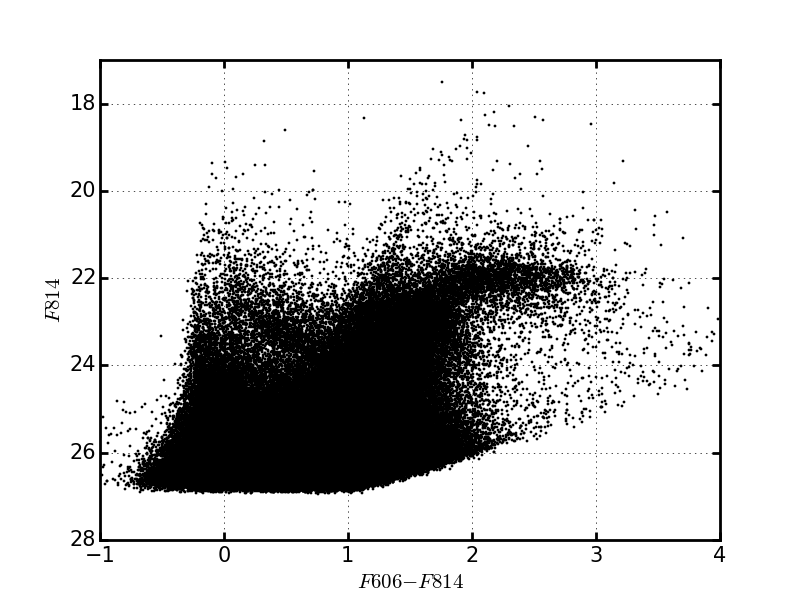
\includegraphics[width=0.65\textwidth]{ngc55/ngc55_V_I}
 \caption[$V-I$ against $V$ colour magnitude diagram for an NGC\,55 field]{
          Colour magnitude diagram for the NGC\,55 optical photometry from the Araucaria Project~\cite{2005Msngr.121...23G}.
          \textbf{placeholder! -- currently this is from the ANGST data}
         }
 \label{fig:VI}
\end{figure}

\begin{figure}
 \centering
 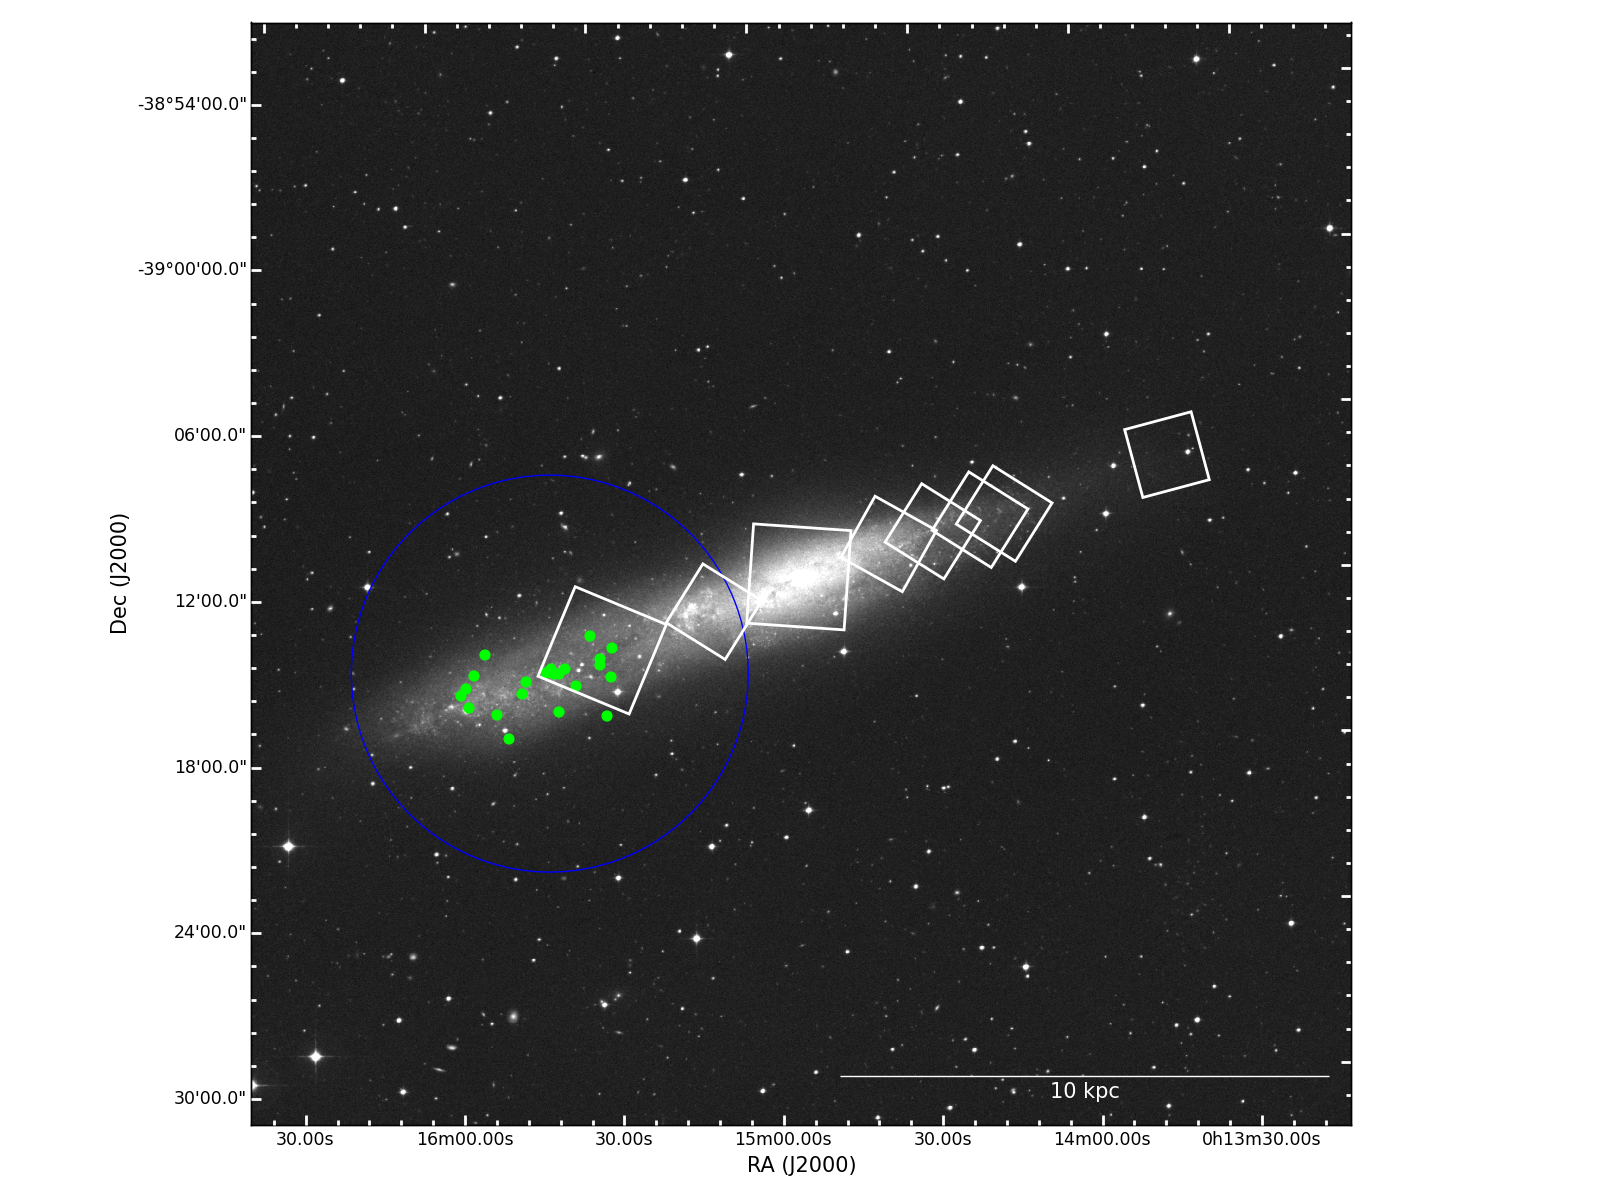
\includegraphics[width=0.65\textwidth]{ngc55/ngc55_fields-v2}
 \caption[Image of NGC\,55 with KMOS and photometric footprints highlighted]{
          Image of NGC\,55 with KMOS targets overlaid in green and photometric footprints from the Araucaria Project
          \protect\citep{2005Msngr.121...23G} in xx
          and the ANGST project
          \protect\citep{2009ApJS..183...67D} in white.
          \textbf{placeholder! Should do this properly and overlay the regions etc on the pretty eso image.}
         }
 \label{fig:ngc55}
\end{figure}

\begin{sidewaystable}
\caption[Summary of VLT-KMOS targets in NGC\,55]{Summary of VLT-KMOS targets in NGC\,55.\label{tb:n55obs-params}}
\scriptsize
\begin{threeparttable}
\centering
\begin{tabular}{lrcccccccccl}
 \hline
 \hline
ID & S/N & $\alpha$ (J2000) & $\delta$ (J2000) & $V$ & $I$ & $F606$ & $F814$ & \multicolumn{3}{c}{$rv$} (\kms) & Notes \\
& &  & & & & & & 16-10-2013 & 14-09-2014 & 15-09-2014\\

 \hline
NGC55-RSG19 & xx & 00:15:29.190 & $-$39:14:08.20& V & 17.73 & F606 & F814 & 178\,$\pm$\,7  & 221\,$\pm$\,10 & 195\,$\pm$\,9 & Notes\\
NGC55-RSG20 & xx & 00:15:29.520 & $-$39:15:13.00& V & 18.95 & F606 & F814 & 195\,$\pm$\,17 & \ldots & \ldots & Notes\\
NGC55-RSG22 & xx & 00:15:30.520 & $-$39:16:36.70& V & 18.56 & F606 & F814 & -17\,$\pm$\,16 & \ldots & \ldots & Notes\\
NGC55-RSG24 & xx & 00:15:31.460 & $-$39:14:46.30& V & 18.48 & F606 & F814 & 194\,$\pm$\,6  & 146\,$\pm$\,38 & 206\,$\pm$\,9 & Notes\\
NGC55-RSG25 & xx & 00:15:31.490 & $-$39:14:32.40& V & 18.39 & F606 & F814 & 217\,$\pm$\,15 & -341\,$\pm$\,29 & 209\,$\pm$\,12 & Notes\\
NGC55-RSG26 & xx & 00:15:33.160 & $-$39:13:42.00& V & 17.96 & F606 & F814 & 173\,$\pm$\,7  & \ldots & \ldots & Notes\\
NGC55-RSG28 & xx & 00:15:36.160 & $-$39:15:29.40& V & 18.99 & F606 & F814 & 161\,$\pm$\,19 & \ldots & \ldots & Notes\\
NGC55-RSG30 & xx & 00:15:38.030 & $-$39:14:50.20& V & 18.73 & F606 & F814 & 215\,$\pm$\,9  & -423\,$\pm$\,21 & 216\,$\pm$\,12 & Notes\\
NGC55-RSG35 & xx & 00:15:39.260 & $-$39:15:01.70& V & 17.87 & F606 & F814 & 206\,$\pm$\,4  & 223\,$\pm$\,12 & 214\,$\pm$\,3 & Notes\\
NGC55-RSG36 & xx & 00:15:39.520 & $-$39:16:23.10& V & 18.46 & F606 & F814 &-284\,$\pm$\,15 & -615\,$\pm$\,28 & 194\,$\pm$\,21 & Notes\\
NGC55-RSG39 & xx & 00:15:40.260 & $-$39:15:01.00& V & 17.97 & F606 & F814 & 192\,$\pm$\,5  & 23\,$\pm$\,23 & 187\,$\pm$\,6 & Notes\\
NGC55-RSG43 & xx & 00:15:40.700 & $-$39:14:50.20& V & 18.18 & F606 & F814 & 196\,$\pm$\,5  & 172\,$\pm$\,16 & 193\,$\pm$\,7 & Notes\\
NGC55-RSG46 & xx & 00:15:41.640 & $-$39:14:58.80& V & 18.44 & F606 & F814 & 208\,$\pm$\,12 & -128\,$\pm$\,17 & -119\,$\pm$\,29 & Notes\\
NGC55-RSG57 & xx & 00:15:45.590 & $-$39:15:16.40& V & 18.22 & F606 & F814 & 197\,$\pm$\,5  & 207\,$\pm$\,13 & 178\,$\pm$\,5 & Notes\\
NGC55-RSG58 & xx & 00:15:46.270 & $-$39:15:43.20& V & 18.40 & F606 & F814 & 216\,$\pm$\,3  & 214\,$\pm$\,21 & 223\,$\pm$\,12 & Notes\\
NGC55-RSG60 & xx & 00:15:49.180 & $-$39:17:19.80& V & 18.85 & F606 & F814 & 26 \,$\pm$\,25 & -500\,$\pm$\,30 & 349\,$\pm$\,30 & Notes\\
NGC55-RSG65 & xx & 00:15:51.250 & $-$39:16:26.40& V & 17.65 & F606 & F814 & 215\,$\pm$\,3  & 217\,$\pm$\,5 & 204\,$\pm$\,6 & Notes\\
NGC55-RSG67 & xx & 00:15:53.110 & $-$39:14:13.60& V & 18.05 & F606 & F814 & 33 \,$\pm$\,21 & 50\,$\pm$\,25 & 28\,$\pm$\,32 & Notes\\
NGC55-RSG69 & xx & 00:15:55.280 & $-$39:15:00.10& V & 18.67 & F606 & F814 & 195\,$\pm$\,8  & 129\,$\pm$\,14 & 202\,$\pm$\,36 & Notes\\
NGC55-RSG70 & xx & 00:15:56.310 & $-$39:16:08.60& V & 18.91 & F606 & F814 & 187\,$\pm$\,8  & 202\,$\pm$\,19 & 184\,$\pm$\,15 & Notes\\
NGC55-RSG71 & xx & 00:15:56.900 & $-$39:15:27.50& V & 18.56 & F606 & F814 & 214\,$\pm$\,10 & 319\,$\pm$\,15 & 256\,$\pm$\,32 & Notes\\
NGC55-RSG73 & xx & 00:15:57.710 & $-$39:15:41.50& V & 18.41 & F606 & F814 & 178\,$\pm$\,5  & 106\,$\pm$\,26 & 182\,$\pm$\,11 & Notes\\

\hline
\end{tabular}
\begin{tablenotes}
  \item Ground based data from the Araucaria Project
  \protect\cite{2006AJ....132.2556P}, with typical photometric uncertainty 0.01 and 0.01 in $V$ and $I$ bands respectively.
  Supplementary ANGST data from
  \protect\cite{2009ApJS..183...67D}, with typical errors 0.015, 0.010, 0.012, in $J, H$ and $K$ bands respectively.
\end{tablenotes}
\end{threeparttable}
\end{sidewaystable}

% subsection target_selection (end)

% section observations (end)

\section{Data Reduction} % (fold)
\label{sec:data_reduction}

The data reduction was performed with the KMOS/esorex pipeline with a several corrections to improve the quality of the reductions which are fully described and characterised in Turner et al. (in prep).

\begin{itemize}
    \item Split recombined sky frames into seeing bins
    \item combine by including pixel shifts between reconstructed IFUs to ensure all frames are correctly matched
    \item etc.
\end{itemize}

Would it be useful to use Skycorr to subtract the sky as in Gazak et al. (2015)

Telluric correction has been performed by combining and reconstrucitng the telluric standard exposures using the standard pipeline routines.
To improve the performance of the telluric correction I use the method described in detail in Chapter~\ref{ch:n6822}.

As mentioned above, were multiple standard star OBs for each night of observing.
The telluric spectrum used to correct each science spectrum is determined on a star-by-star basis depending upon a visual inspection of the results of the correction.

% section data_reduction (end)

\section{Results} % (fold)
\label{sec:results}

\subsection{Radial Velocities} % (fold)
\label{sub:rvs}
Radial velocities are measured using the method described first in Chapter~\ref{ch:n2100}.
This method is known to work well on KMOS stellar spectra from previous studies~\cite{2015ApJ...798...23L,2015ApJ...803...14P,2016arXiv160202702P}.
Estimated radial velocities from each KMOS pointing is listed in Table~\ref{tb:n55obs-params}.

Distance modulus~=~26.58\,$\pm$\,0.11~\citep{2011ApJ...738..150T}

\begin{itemize}
    \item Association with NGC\,55
    \item Does this desrve a subsection of its own?
    \item Radial velocity Vs. Radius from galaxy centre
    \item Comparison with previous estimates for these stars and galaxy wide
\end{itemize}

\begin{figure}
 \centering
 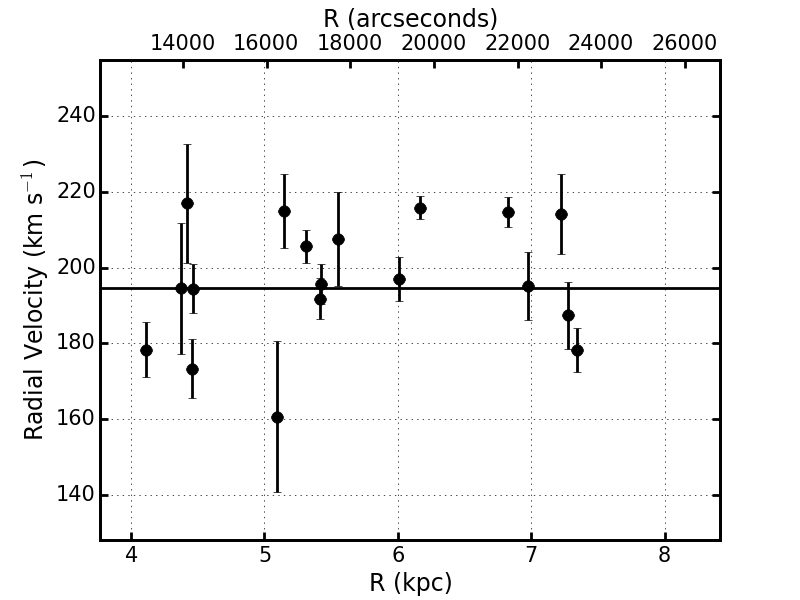
\includegraphics[width=0.65\textwidth]{ngc55/ngc55-RvsRV-F1}
 \caption[Radial velocities for the KMOS RSGs shown against projected radius]{
 Radial velocities for the KMOS RSGs shown against projected radius
         }

 \label{fig:ngc55}
\end{figure}
% subsection radial_velocities (end)
\subsection{Stellar Parameters} % (fold)
\label{sub:stellar_parameters}
\begin{itemize}
    \item Comparison to previous results
    \item [Z] Vs. Radius from galaxy centre
    \item MCMC parameter estimation for the fit
    \end{itemize}

% subsection stellar_parameters (end)

% section results (end)

\section{Discussion} % (fold)
\label{sec:discussion}

\begin{itemize}
    \item Orientation of NGC\,55
\end{itemize}
% section discussion (end)

\section{Conclusions} % (fold)
\label{sec:conclusions}

% section conclusions (end)





\appendix
\addtocontents{toc}{\protect\tocappendix}
% \chapter{The First Appendix}

Lorem ipsum dolor sit amet, consectetur adipiscing elit. Sed adipiscing porttitor turpis sed congue. Phasellus ac magna mi. Vivamus et dolor justo. Vivamus ligula dolor, consequat et sodales eget, mattis at ligula. Nulla arcu nisi, porttitor a ornare eget, luctus eget mi. Vivamus adipiscing turpis in ligula tempus blandit. Vestibulum rutrum sodales quam, quis blandit mauris sollicitudin in. Maecenas lacinia gravida velit nec venenatis. Curabitur eget orci aliquet augue adipiscing bibendum. Sed in tortor metus. Ut sit amet nisl odio. Maecenas accumsan, mauris a auctor egestas, nisl ante imperdiet arcu, ac volutpat erat neque rutrum turpis. Pellentesque ut est et lectus interdum fringilla sit amet non purus. Aliquam erat volutpat. Etiam rhoncus, leo vel facilisis lacinia, quam augue ultricies dui, nec feugiat nunc sapien quis diam.


\backmatter

\singlespace

% \phantomsection
% \addcontentsline{toc}{chapter}{\bibname}
% Choose a bibliography style to suit your taste here
% This one was downloaded from http://web.reed.edu/cis/help/latex/bibtexstyles.html (June 2012)
% \bibliographystyle{mn2e}
% \bibliography{journals}

\end{document}
